% Template copied from Brooke Simmons' draft of the GZ-CANDELS bar paper


\documentclass[useAMS,usenatbib]{mn2e}
%\documentclass[twocolumn]{emulateapj}
\usepackage{graphicx,natbib,color,multirow,amsmath}
\bibliographystyle{mn2e}
\voffset=-0.8in

\definecolor{titlecol}{rgb}{0,0,1}
\definecolor{titlecol2}{rgb}{0,0.65,0}
\definecolor{darkorange}{rgb}{0.85,0.37,0.05}

%\definecolor{titledark}{rgb}{0,0,0.8}
%\definecolor{hilit}{rgb}{0,0,1}
%\definecolor{hilitdark}{rgb}{0,0,0.8}
%\font\sbf=cmssbx10 at 32.28pt %big font for headers

\font\nbf=cmssbx10 at 12.28pt %big font for headers

%%%%%%%%%%%%%%%%%%%%%%%%%%%%%%%
%%%% If you want to leave notes in the text feel free to define
%%%% your own colour above and a style below
%%%%%%%%%%%%%%%%%%%%%%%%%%%%%%%
\def\note		{\color{titlecol2} \nbf}
\def\noteb		{\color{titlecol} \nbf}
\def\notebsm	{\color{titlecol}}
\def\notec		{\color{titlecol2} \nbf}
\def\notek		{\color{darkorange} \nbf}

%%%%%%%%%%%%%%%%%%%%%%%%%%%%%%%
% For the eventual referee response
\def\changed    {\color{titlecol} }
%\def\changed    {}


%%%%%%%%%%%%%%%%%%%%%%%%%%%%%%%
%  Other stuff I use a lot
\def\oiii		{$\mathrm{\left[ O \textsc{iii}\right] }$}
\def\moiii		{\mathrm{\left[ O \textsc{iii}\right] }}
\def\nii		{$\mathrm{\left[ N \textsc{ii}\right] }$}
\def\mnii		{\mathrm{\left[ N \textsc{ii}\right] }}
\def\sii		{$\mathrm{\left[ S \textsc{ii}\right] }$}
\def\msii		{\mathrm{\left[ S \textsc{ii}\right] }}
\def\galfit     {{\tt GALFIT}}

\def\mmsun	{\rm{M}_{\odot}}
\def\fnobulge    {$f_{\rm no~bulge}$}
\def\mfnobulge {f_{\rm no~bulge}}
\def\fedgeon     {$f_{\rm edge-on}$}
\def\mfedgeon  {f_{\rm edge-on}}
\def\fcnobulge    {$f_{\rm confirmed~no~bulge}$}
\def\mfcnobulge {f_{\rm confirmed~no~bulge}}

% Fixes for the journal abbreviations in bibtex file
\newcommand{\mnras}{MNRAS}
\newcommand{\apj}{ApJ}
\newcommand{\aj}{AJ}
\newcommand{\apjl}{ApJL}
\newcommand{\apjs}{ApJS}
\newcommand{\aap}{A\&A}
\newcommand{\araa}{ARA\&A}
\newcommand{\pasp}{PASP}
\newcommand{\fcp}{Fund. Cosm. Phys.}


%\def\lesssim{\mathrel{\hbox{\rlap{\hbox{\lower5pt\hbox{$\sim$}}}\hbox{$<$}}}}
%\def\gtrsim{\mathrel{\hbox{\rlap{\hbox{\lower5pt\hbox{$\sim$}}}\hbox{$>$}}}}
%new defs of lesssim gtrsim that I think look better
\def\lesssim{\mathrel{\hbox{\rlap{\hbox{\lower3pt\hbox{$\sim$}}}\hbox{\raise2pt\hbox{$<$}}}}}
\def\gtrsim{\mathrel{\hbox{\rlap{\hbox{\lower3pt\hbox{$\sim$}}}\hbox{\raise2pt\hbox{$>$}}}}}


\newcommand\nodata{ ~$\cdots$~ }


\begin{document}

\title[Galaxy Zoo-UKIDSS : near-infrared morphologies for galaxies in the local Universe]{Galaxy Zoo-UKIDSS : near-infrared morphologies\thanks{This publication has been made possible by the participation of more than 200,000 volunteers in the Galaxy Zoo project.} } \author[Willett et al.]{\parbox[t]{16cm}{Willett, Schawinski, Simmons, Lintott, Masters, Edmondson, Keel, Fortson, GZ, UKIDSS, et~al.; \underline{{\it name order/inclusion not at all fixed}}
\vspace{0.1in} }\\
$^{1}$School of Physics and Astronomy, University of Minnesota, 116 Church St. SE, Minneapolis, MN 55455, USA\\
$^{2}$Oxford Astrophysics, Denys Wilkinson Building, Keble Road, Oxford OX1 3RH, UK\\
% All or most of these will be needed later
%$^{2}$Yale Center for Astronomy and Astrophysics, Yale University, P.O. Box 208121, New Haven, CT 06520, USA\\
%$^{3}$Department of Astronomy, Yale University, New Haven, CT 06511, USA\\
%$^{4}$Adler Planetarium, 1300 S. Lake Shore Drive, Chicago, IL 60605, USA\\
%$^{5}$Department of Physics, Yale University, New Haven, CT 06511, USA\\
%$^{6}$Astronomy Department, Wesleyan University, Middletown, CT 06459, USA\\
%$^{7}$Blackett Laboratory, Imperial College London, London SW7 2AZ, UK\\
%$^{8}$Institute of Cosmology \& Gravitation, University of Portsmouth, Dennis Sciama Building, Portsmouth PO1 3FX, UK\\
%$^{9}$SEPnet,\thanks{www.sepnet.ac.uk} South East Physics Network, School of Physics \& Astronomy, University of Southampton, HighÞeld, Southampton SO17 1BJ, UK\\
%$^{11}$Centre for Astronomy and Particle Theory, The University of Nottingham, University Park, Nottingham NG7 2RD, UK
   }
  
\maketitle
  
\label{firstpage}
  
\begin{abstract}

GZ-UKIDSS: the abstract. 

\end{abstract}
  
\begin{keywords}

    galaxies: bars 
    --- 
    galaxies: evolution
    --- 
    galaxies: general 
    --- 
    galaxies: spiral 

\end{keywords}

%%%%%%%%%%%%%%%%%%%%%%%%%%%%%%%%%%%%%%%%%%%%%%
%
%  
\section{Introduction}
%
%
%%%%%%%%%%%%%%%%%%%%%%%%%%%%%%%%%%%%%%%%%%%%%%

% This 1st paragaph is SO stolen from Brooke. Must change.
Because galactic stellar bars form only within dynamically cold, rotationally supported disks \citep{com09a,ath13}, the evolution of the fraction of disk galaxies with bar features traces the overall evolution of disk galaxy dynamics. Locally, bars are present in $\sim 25 - 50\%$ of disk galaxies \citep[e.g.][]{mas11c,agu09}, with their abundance steadily decreasing to $\sim$10\% of disk galaxies at $z \sim 1$ \citep{she08a, elm04}. 

However, these results have shown that the observed bar fraction in large samples of galaxies has a strong dependence on the observing wavelength. Optical studies consistently reveal results toward the lower end of this range \citep{mas11c}, while infrared results uncover older stellar populations that trace the bar potential in larger numbers of galaxies \citep{she08a}. As a result, it is critical for cosmological studies that the rest frame of the galaxies remain constant as a function of redshift (see Melvin et al. 2014 in press, Simmons et al. 2014 in prep). 

In this paper, we use combine previous optical studies of bars in the local Universe collected by the Galaxy Zoo 2 (GZ2) project \citep{wil13} with new classifications in the infrared. The new images were taken with the United Kingdom Infrared Telescope (UKIRT) as part of the UKIRT Infrared Deep Sky Survey \citep[UKIDSS;][]{law07,war07}. The Large Area Survey (LAS) portion of UKIDSS covered the SDSS observations at high Galactic latitudes, allowing for \emph{YZJHK} coverage for 71,052 galaxies that had also been classified in GZ2. This paper compares the optical and infrared morphologies of these galaxies and study the evolution of their overall bar fraction as a function of wavelength and colour. 

In Section~\ref{sec:data} we describe the sample selection, including a summary of Galaxy Zoo 2 classifications of UKIDSS galaxies and the identification of bars in non-inclined disks. We also explore any potential biases that may affect our results. We present our results in Section~\ref{sec:results}, with discussion in Section~\ref{sec:discussion} and a summary in Section~\ref{sec:conclusions}. 

This paper uses a cosmology consistent with $\Lambda$CDM, having $H_{\rm 0}=70~{\rm
km~s^{-1}}$Mpc$^{\rm -1}$, $\Omega_{\rm m}=0.3$ and $\Omega_{\rm \Lambda}=0.7$ \citep{ben13,pla13}.

%Should make clear somewhere here that this is a first look at the GZ-UKIDSS classifications.



%%%%%%%%%%%%%%%%%%%%%%%%%%%%%%%%%%%%%%%%%%%%%%
%
%
\section{Data}\label{sec:data}
%
%
%%%%%%%%%%%%%%%%%%%%%%%%%%%%%%%%%%%%%%%%%%%%%%

\subsection{UKIDSS}\label{sec:ukidss_data}

Details about UKIDSS area coverages and depth.

Number of objects total above some flux limit, from which we have visual classifications from the Galaxy Zoo project.


\subsection{SDSS}\label{sec:sdss_data}


\subsection{Morphological classifications}\label{sec:gz_data}

The Galaxy Zoo project provides quantified visual classifications of galaxies by obtaining multiple independent classifications for each galaxy. Beginning in 2007, more than 1,000,000 galaxy images total from both the Sloan Digital Sky Survey and the \emph{Hubble Space Telescope} were each classified by $\sim 40$ independent volunteers via a web interface\footnote{www.galaxyzoo.org}. The initial version of the project \citep{lin08,lin11} asked a single question per galaxy; subsequent versions have collected more detailed morphological information, including finer sub-structures of disk galaxies such as bulge strength and bars, via a tiered classification tree \citep[e.g.,][]{wil13}. 

This work uses classifications collected during the second release of the project: Galaxy Zoo 2. % More details about number, selection, etc.

The classification tree used for GZ-UKIDSS is identical to that in GZ2, precisely so that the two datasets can be compared using the same morphological definitions. The tiered decision tree \citep{wil13} first asks volunteers to choose whether a galaxy is mostly smooth, has features, or is a star/artifact. The bar classification question (``Is there a sign of a bar feature through the centre of the galaxy?'') is reached once a volunteer has chosen ``Features or Disk'' as an answer to the first question and has subsequently said the galaxy is \emph{not} an edge-on disk. The bar vote is therefore a third-tier question, and the number of volunteers per galaxy who answer the question varies depending on each volunteer's answers to the earlier questions about the galaxy.

What are average number of answers $N$ for the bar classification question overall? In non-edge-on disks?

\subsection{Sample selection}\label{sec:sample}

%%%%% [FIGURE: GZ2 vs. UKIDSS bar fractions] %%%%%
\begin{figure*}
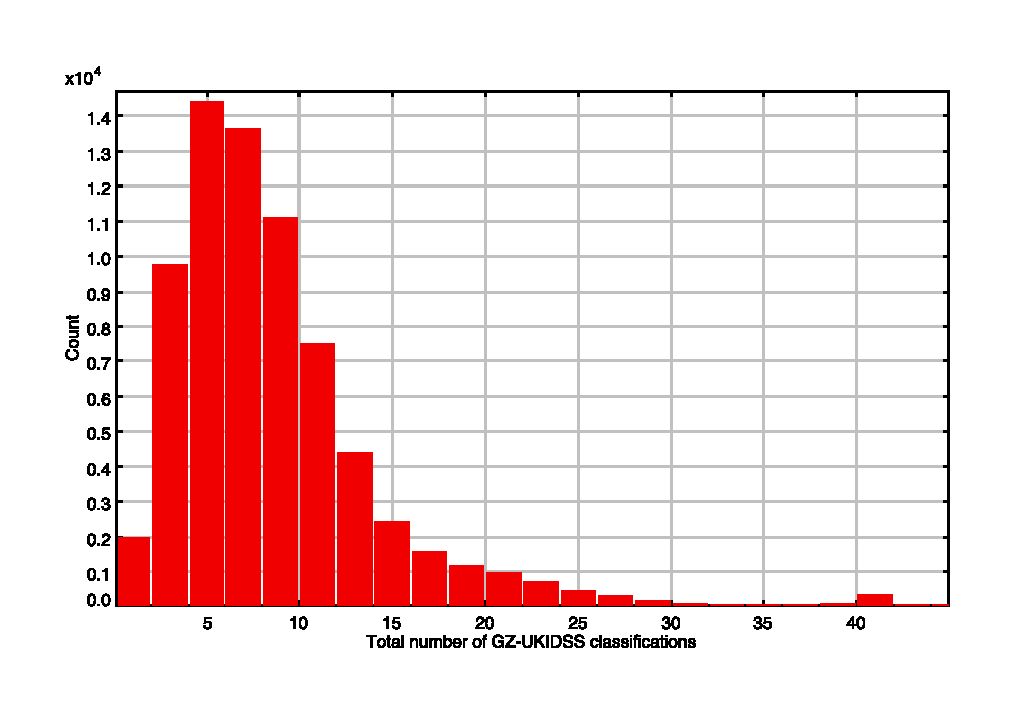
\includegraphics[scale=1.0]{figures/ukidss_count.eps}
\caption{
    Total number of classifications in GZ-UKIDSS as of 12-Jan-2014. The median is 7 and mean 7.9 classifications per galaxy, with a long tail stretching out (log-normal distribution?) to $N=44$. I do not know whether there is an active retirement algorithm in place for the UKIDSS images. Preliminary results suggest we will need at least 40~classifications per galaxy, though, since the shot noise for even relatively high-level questions is quite high. 
}
\label{fig:ukidss_count}
\end{figure*}
%%%%%% END FIGURE %%%%%

%%%%%% END FIGURE %%%%%

%%%%% [FIGURE: GZ2 vs. UKIDSS features/disk fractions] %%%%%
\begin{figure*}
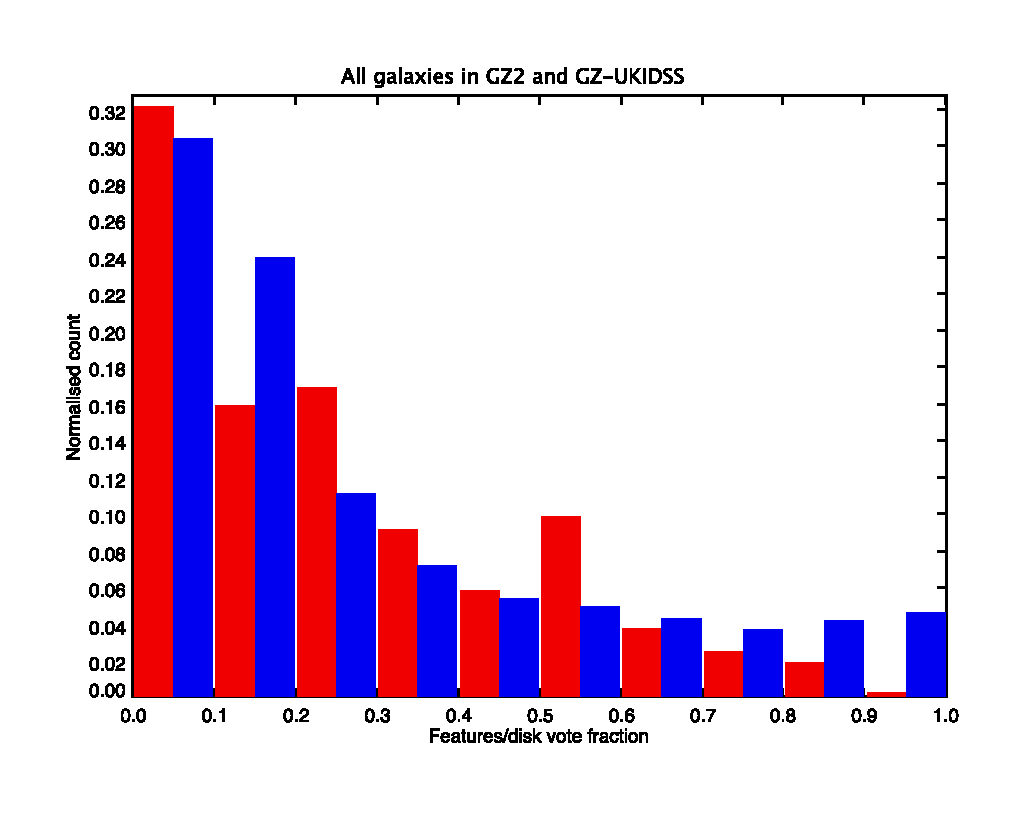
\includegraphics[scale=1.0]{figures/features_histogram.eps}
\caption{
    Distribution of the fraction of galaxies with features or disks ($f = N_{features/disk}/N_{classifications}$) in both {\bf\color{red}UKIDSS} and {\bf\color{blue}GZ2}. UKIDSS galaxies have significantly fewer examples of feature/disk-dominated morphology than their GZ2 counterpart classifications, especially at $f>0.9$. This sample contains 53,868 galaxies (note: this should match the entire GZ-UKIDSS sample of 71,052 galaxies; not yet sure why some aren't showing up in both). 
}
\label{fig:features_histogram}
\end{figure*}
%%%%%% END FIGURE %%%%%

%%%%% [FIGURE: GZ2 vs. UKIDSS bar fractions] %%%%%
\begin{figure*}
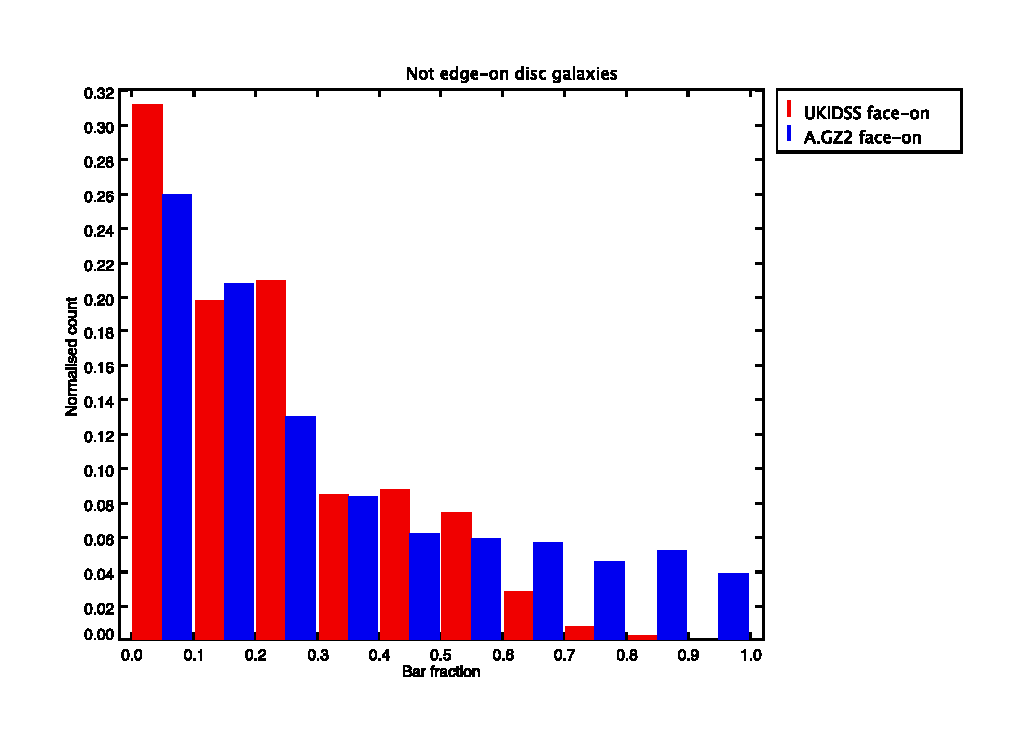
\includegraphics[scale=1.0]{figures/bar_fraction_histogram.eps}
\caption{
    Distribution of the bar fraction ($N_{bar}/N_{not edgeon disks}$) in both {\bf\color{red}UKIDSS} and {\bf\color{blue}GZ2}. The distributions are similar for low and intermediate bar fractions; however, UKIDSS has virtually no galaxies above a bar fraction of 0.7 (a common ``clean'' threshold in GZ1 and GZ2). The bar fraction is only measured for disk galaxies with $N_{classifications} \geq 10$, $f_{features/disk} \geq 0.2$, and $f_{not edgeon}\geq0.5$; this is 1,178 galaxies, or 2\% of the total sample. These disk galaxy criteria are significantly lower than those in GZ2 ($N_{classifications} \geq 20$, $f_{features/disk} \geq 0.430$, and $f_{not edgeon}\geq0.715$). 
}
\label{fig:bar_fraction_histogram}
\end{figure*}
%%%%%% END FIGURE %%%%%

%%%%% [FIGURE: GZ2 vs. UKIDSS bar fractions] %%%%%
\begin{figure*}
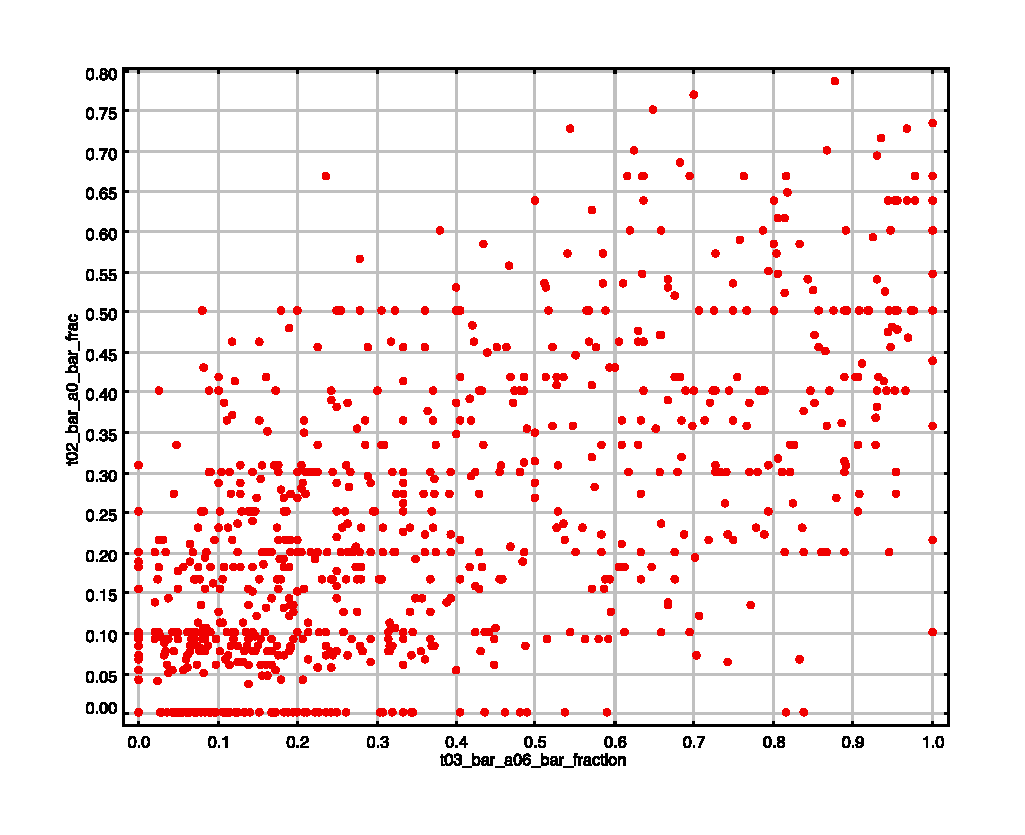
\includegraphics[scale=1.0]{figures/scatter.eps}
\caption{
    Bar fractions for matched disk galaxies classified in both GZ2 and GZ-UKIDSS (same as Figure~\ref{fig:bar_fraction_histogram}). The data have a Spearman's correlation coefficient of $\rho=0.612$; this is statistically significant ($p<10^{-85}$), but clearly the scatter is enormous. The best-fit line has a slope less than 1, consistent with the lack of strongly-identified bars in GZ-UKIDSS. Interestingly, there are very few galaxies in the upper left, which would be undetected in the optical and appearing in the infrared. This contradicts some of the initial expectations of the GZ-UKIDSS project and the higher bar fractions ($\sim65\%$) measured in infrared studies \citet{why02,mar07a,men07a,she08a} compared to optical \citep{bar08,mas11c,lee12}.
}
\label{fig:scatter}
\end{figure*}
%
%%%%% [FIGURE: GZ2 vs. UKIDSS bar fraction images] %%%%%
\begin{figure*}
\includegraphics[scale=0.6]{figures/bar_decreasing_images.pdf}
\caption{
    Example \emph{YHK} images for various values of $f_{bar}$ of GZ-UKIDSS disk galaxies (not edge-on). Starting in the top left and moving down, then rightward to the bottom right, the vote fraction for bars goes from $f_{bar}=0.785$ (the highest in the matched category) to $f_{bar}=0$. Interestingly, there are visible bars (according to experts KS and KWW) in almost all these randomly-selected images, and down to vote fractions as low as $f_{bar}=0.1$. This suggests that GZ-UKIDSS classifiers have a much lower threshold for possible bar identification than GZ2, and \emph{must} be evaluated with different criteria.
}
\label{fig:images}
\end{figure*}
%
%%%%% [FIGURE: GZ2 vs. UKIDSS, very different] %%%%%
\begin{figure*}
\includegraphics[scale=0.6]{figures/bars_different_gz2_ukidss.pdf}
\caption{
    Example \emph{YHK} images for two galaxies with very different bar classifications in GZ2 and GZ-UKIDSS. The top galaxy is a strong bar in the optical and a very weak bar in the infrared ($f_{bar,GZ2}=1.0$, $f_{bar,UKIDSS} = 0.1$). The bottom galaxy is a strong bar in the infrared and weak bar in the optical ($f_{bar,GZ2}=0.235$, $f_{bar,UKIDSS} = 0.667$). These represent the extreme examples of galaxies in the lower right and upper left corners, respectively, of Figure~\ref{fig:scatter}. 
}
\label{fig:different}
\end{figure*}
%
A full reduction of the GZ-UKIDSS classifications, resulting in a catalog of morphological vote fractions for each galaxy, is ongoing. Here we use the raw vote fractions, which have been neither weighted nor debiased \citep[by a procedure similar to][]{wil13}. We also use the raw GZ2 vote fractions for strict comparison, rather than the ``debiased'' data products available from \citet{wil13}. The effects of using raw versus the reduced classifications are twofold. First, the unweighted vote fractions are likely biased in the first question toward an excess of votes for ``Star or Artifact''. Second, the effects of surface brightness dimming are not accounted for in the vote fractions, which is a minor effect for galaxies in which disk structure is previously identified and within a relatively small spatial volume ($z<0.1$). 

To minimize the impact of the lack of user weighting, we employed a lower vote fraction threshold when selecting ``featured'' galaxies compared to thresholds using weighted data. We select as ``featured'' galaxies those where at least 20\% of votes (out of at least 10 volunteers total) were registered for ``Features or Disk''. After the first question, the user weighting used by previous Galaxy Zoo data reductions affects vote fractions by typically no more than a few percent; we therefore expect the lack of weighting to have little to no systematic effect on additional vote fractions. 

Further, we also require that 50\% of volunteers (of at least 10) registered a vote for not-edge-on. 

%%%%%%%%%%%%%%%%%%%%%%%%%%%%%%%%%%%%%%%%%%%%%%
%
%
\section{Results: Bar fractions}\label{sec:results}
%
%
%%%%%%%%%%%%%%%%%%%%%%%%%%%%%%%%%%%%%%%%%%%%%%


%%%%%%%%%%%%%%%%%%%%%%%%%%%%%%%%%%%%%%%%%%%%%%
%
%  
\section{Discussion}\label{sec:discussion}
%
%
%%%%%%%%%%%%%%%%%%%%%%%%%%%%%%%%%%%%%%%%%%%%%%

%%%%%%%%%%%%%%%%%%%%%%%%%%%%%%%%%%%%%%%%%%%%%%
%
%  
\section{Conclusions}\label{sec:conclusions}
%
%
%%%%%%%%%%%%%%%%%%%%%%%%%%%%%%%%%%%%%%%%%%%%%%

%%%%%%%%%%%%%%%%%%%%%%%%%%%%%%%%%%%%%%%%%%%%%%
%
%
\section*{Acknowledgments}
%
%
%%%%%%%%%%%%%%%%%%%%%%%%%%%%%%%%%%%%%%%%%%%%%%

%
The JavaScript Cosmology Calculator \citep{wri06} and TOPCAT \citep{tay05,tay11} were used while preparing this paper. 
%
KWW acknowledges support from the NSF under grant DRL-0941610.
%
\textbf{Please send your grant acknowledgments at your earliest convenience.}
%
Galaxy Zoo was supported by The Leverhulme Trust. 

%%%%%%%% UKIDSS ACKNOWLEDGMENT                  (NEED)

Funding for the SDSS and SDSS-II has been provided by the Alfred P. Sloan Foundation, the Participating Institutions, the National Science Foundation, the U.S. Department of Energy, the National Aeronautics and Space Administration, the Japanese Monbukagakusho, the Max Planck Society, and the Higher Education Funding Council for England. The SDSS Web Site is http://www.sdss.org/.

The SDSS is managed by the Astrophysical Research Consortium for the Participating Institutions. The Participating Institutions are the American Museum of Natural History, Astrophysical Institute Potsdam, University of Basel, University of Cambridge, Case Western Reserve University, University of Chicago, Drexel University, Fermilab, the Institute for Advanced Study, the Japan Participation Group, Johns Hopkins University, the Joint Institute for Nuclear Astrophysics, the Kavli Institute for Particle Astrophysics and Cosmology, the Korean Scientist Group, the Chinese Academy of Sciences (LAMOST), Los Alamos National Laboratory, the Max-Planck-Institute for Astronomy (MPIA), the Max-Planck-Institute for Astrophysics (MPA), New Mexico State University, Ohio State University, University of Pittsburgh, University of Portsmouth, Princeton University, the United States Naval Observatory, Yale University and the University of Washington. 
  
\bibliography{kwrefs}  

\end{document}
